% use ACM template style
\documentclass{sig-alternate}

%set it to Spanish
\usepackage[spanish]{babel}
%\usepackage[dvips]{epsfig}     % To include PostScript
\usepackage{xcolor,graphicx}
\usepackage{url}
\usepackage[pdftex]{hyperref}
%code highlight
\usepackage{listings}
\lstset{
basicstyle=\small\sffamily,
frame=tb,
columns=fullflexible,
showstringspaces=false
}
% URLs in different colors	
\hypersetup{urlcolor=black, citecolor=black, linkcolor=black, colorlinks=true }
\graphicspath{{img/}}

% remove copyright notes from the ACM template
\makeatletter
\def\@copyrightspace{\relax}
\makeatother

\begin{document}
%
% --- Author Metadata here ---
%\conferenceinfo{WOODSTOCK}{'97 El Paso, Texas USA}
%\CopyrightYear{2007} % Allows default copyright year (20XX) to be over-ridden - IF NEED BE.
%\crdata{0-12345-67-8/90/01}  % Allows default copyright data (0-89791-88-6/97/05) to be over-ridden - IF NEED BE.
% --- End of Author Metadata ---

\title{Herramienta de generaci\'on de documentaci\'on: Sphinx-doc}

\numberofauthors{4} %  in this sample file, there are a *total*
% of EIGHT authors. SIX appear on the 'first-page' (for formatting
% reasons) and the remaining two appear in the \additionalauthors section.
%
\author{
% 1st. author
\alignauthor
Carla Villena
       \email{ing.carla.villena@gmail.com}
% 2nd. author
\alignauthor
Marines Lopez\\
       \email{mary.jlm.2006@gmail.com}
% 3rd. author
\alignauthor 
Timoteo Ponce\titlenote{disertante}\\
       \email{ponce.timoteo@gmail.com}\\
\and  % use '\and' if you need 'another row' of author names
% 4th. author
\alignauthor 
	Roger U\~noja\\
       \email{rhunoja@gmail.com}
}

\maketitle
\begin{abstract}
  El proceso de documentaci\'on de un producto y/o proceso 
  es paralelo al desarrollo del mismo, por tanto se deben 
  tratar como tal agregando herramientas que automaticen
  las tareas de documentaci\'on de form automatizada.

  Este art\'iculo provee un an\'alisis inicial a la 
  herramienta de documentaci\'on \emph{Sphinx-doc}, tanto como utilidad
  de generaci\'on de documentos como de gesti\'on de los 
  mismos. Adem\'as indica las operaciones b\'asicas de 
  uso y el proceso de instalaci\'on del mismo, incluyendo 
  los pasos necesarios para la creaci\'on de un proyecto
  de documentaci\'on.

\end{abstract}

% A category with the (minimum) three required fields
\category{Software Engineering}{Knowledge Management}[analysis, installation]
%A category including the fourth, optional field follows...
%\category{D.2.8}{Software Engineering}{Metrics}[complexity measures, performance measures]

\terms{Tools}

\keywords{Markup, documentation, installation, configuration, an\'alysis}

\section{Introducci\'on}

  \emph{Sphinx-doc} es una herramienta de gesti\'on y generaci\'on 
  de documentaci\'on de prop\'osito general desarrollada para 
  soportar la sintaxis simple de texto plano \emph{reStructuredText}. 
  Su accesabilidad es abierta debido a su licencia de c\'odigo abierto
  y su aplicabilidad se expande a los mismos dominos de Python, 
  ya que est\'a escrita en ese lenguaje base.
  \\ \\
  El proceso de generaci\'on de documentos que realiza inicia con 
  el contenido de los mismo elaborados en formato \emph{reStructuredText}, 
  luego \emph{Sphinx-doc} utiliza un parser interno para generar una 
  representaci\'on l\'ogica de ese contenido el cual posteriormente 
  ser\'a exportado a uno o varios de los m\'ultiples formatos 
  que soporta \cite{sphinx0}.
  \\ 
  \begin{figure}[!htbp]
        \centerline{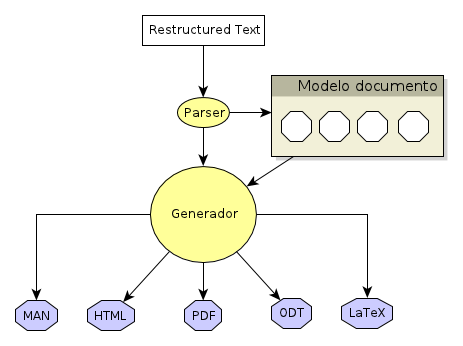
\includegraphics[height=5cm]{sphinx_model.png}}
	\caption{Proceso de generaci\'on de contenidos}
  \end{figure}
  
\section{Caracter\'isticas}

  \begin{itemize}
   	\item Completamente basado en texto, usando una sintaxis \emph{reStructuredText}.
   	\item Soporte de m\'ultiples formatos:
    	HTML, PDF, Latex, Man pages, Open Document, XML. 
   	\item Multiplataforma, como efecto secundario de su implementaci\'on 
    	en Python.
   	\item Documentaci\'on y referencias disponibles al p\'ublico.
   	\item Comunidad de uso y desarrollo extensa.
	\item Extensibilidad, pueden agregarse extensiones al sistema
	    actual y usarlas indistintamente si ningun problema.
	\item Gesti\'on de proyecto, permite definir a la documentaci\'on
	    como un proyecto con metadatos, versionamiento y una estructura
	    definida para su gesti\'on.
	\item Completamente basado en consola y comandos Make, facilitando
	    la ejecuci\'on de tareas repetitivas.
	\item Integraci\'on, como paquete de software est\'a integrado 
	    en entornos Unix-like a trav\'es de MacPorts, DebPackages y 
	    RPM.
	\item Soporte de plantillas de contenido, permitiendo definir 
	    documentos base para su posterior uso.
	\item Herramientas de validaci\'on autom\'atica de elementos 
	    de la documentaci\'on utilizando scripts y snippets 
	    predeterminados.
	\item Versionamiento, permite diferenciar los elementos modificados,
	    agregaos y eliminados del proyecto.
	\item Validaci\'on, ofrece herramientas automatizadas para validar
	    las referencias internas y externas usadas en los archivos
	    de documentaci\'on: im\'agenes, sitios web, archivos remotos, etc.
  \end{itemize}
  
\section{Instalaci\'on y configuraci\'on}

	Para la instalaci\'on de las utilidades para el uso de \emph{Sphinx-doc} 
	se requiere inicialmente la instalaci\'on de la plataforma base
	Python. Es recomendable instalar \emph{Sphinx-doc} usando el sistema 
	de empaquetamiento de Pytho \cite{sphinx2}.
	
	\subsection{Debian Linux}
		A trav\'es del sistema de paquetes Deb.
		
	\begin{lstlisting}
$> sudo apt-get install 
	\ python python-docutils 
	\ python-setuptools
$> sudo easy_install
	\ -U Sphinx 
	\end{lstlisting}
	
	\subsection{Windows}
		En ambientes Windows su instalaci\'on se limita a la instalaci\'on del paquete 
		completo de Python y la instalaci\'on de \emph{Sphinx-doc} a trav\'es del sistema
		de paquetes de Python.
		\begin{enumerate}
			\item Descargar Python 2.x.
			\item Ejecutar el instalador.
			\item Colocar el directorio de instalaci\'on de Python como 
				parte de la variable global PATH.
			\item Instalar \emph{Sphinx-doc}:
	\begin{lstlisting}
c:> easy_install -U Sphinx 
	\end{lstlisting}
		\end{enumerate}
	
	\subsection{Configuraci\'on de un proyecto}
		
		A continuaci\'on crearemos un proyecto de documentaci\'on en \emph{Sphinx-doc}
		usando \emph{reStructuredText} (todas las operaciones se describen
		para ser ejecutadas desde una terminal o consola):
		
		\begin{enumerate}
			\item Crear una carpeta con el nombre 'doc\_project\_1'.
			\item En la carpeta 'doc\_project\_1' ejecutar 'sphinx-quickstart'
			
\begin{lstlisting}
$> cd doc_project_1
$> sphinx-quickstart
\end{lstlisting}

			\item A continuaci\'on se pediran diferentes valores de configuraci\'on, 
				solamente personalize los de nombre del proyecto, los autores y 
				el n\'umero de versi\'on. Para 
				todos los dem\'as deje los valores por defecto.
\begin{lstlisting}
... 
> Project name: doc_project_1
> Author name(s): Timoteo Ponce
...
> Project version: 1
> Project release [1]: 
...
\end{lstlisting}

			\item Ejecutar el comando 'make html' para generar toda la estructura 
				base en HTML, todos los archivos se encuentran bajo la carpeta 
				'build/html'.
			
\begin{lstlisting}
$> make html
\end{lstlisting}

			\item Agregar el siguiente contenido a un archivo nuevo en 'pagina1.rst'.
			
\begin{lstlisting}
# pagina1.rst
===== 
Titulo 
===== 
Subtitulo 
-------- 
Los titulos son definidos usando 
subrayado con barras horizontales, 
siendo dobles para titulos del nivel 1
y simples para subtitulos.
	
Los parrafos se *separan* **por** una linea 
en blanco. Los caracteres mas comunes 
son "``= - ` : ' " ~ ^ _ * + # < >``". 	
\end{lstlisting}
			\item Vuelva a ejecutar el comando 'make html' para actualizar el contenido
				y rev\'iselo con un navegador web.
		\end{enumerate}

	\begin{figure}[!htbp]
	  \centerline{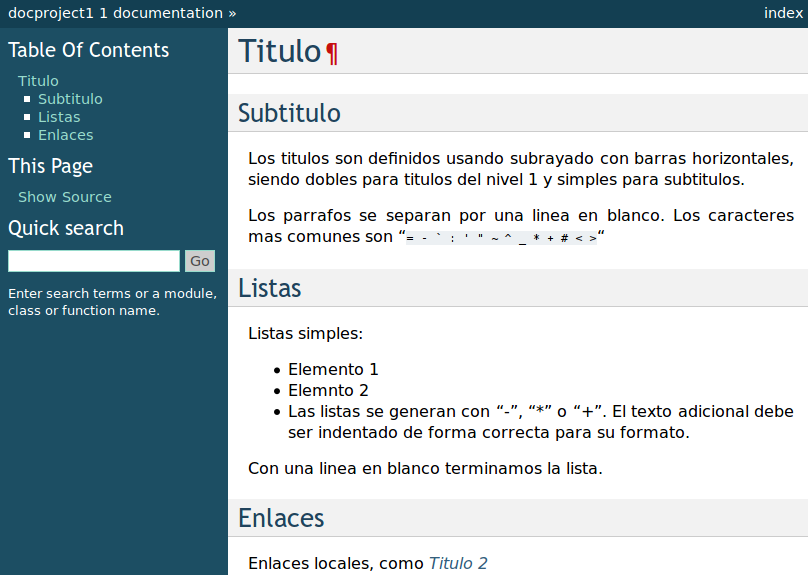
\includegraphics[height=6cm]{rest_1.png}}
	\caption{Contenido generado en HTML}
	\end{figure}


\section{Proyecto de documentaci\'on}

	\emph{Sphinx-doc} genera archivos de configuraci\'on de un proyecto 
	con metadatos necesarios para realizar versionamiento, seguimiento
	y gesti\'on de los artefactos de contenido y exportados en 
	la documentaci\'on, los principales elementos del proyecto 
	son:
	
	\begin{figure}[!htbp]
	  \centerline{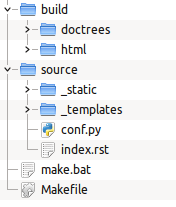
\includegraphics[height=5cm]{dir_structure.png}}
	  \caption{Estructura de directorios \emph{Sphinx-doc}}
	\end{figure}
	
	\begin{itemize}
	 \item \textbf{Makefile}, archivo de construcci\'on
	    autom\'atica para la ejecuci\'on de tareas del proyecto.
	 \item \textbf{make.bat}, script equivalente a Makefile 
	    para entornos Windows.
	 \item \textbf{conf.py}, archivo de propiedades y configuraci\'on
	    del proyecto, en esta parte se colocan todos los metadatos
	    relativos al autor, nombre del proyecto, versi\'on, etc.
	 \item \textbf{index.rst}, archivo de contenido definiendo 
	    la ra\'iz de toda la documentaci\'on. Este archivo define
	    la estructura base para todo el documento.
	 \item \textbf{build/}, directorio predeterminado para todos 
	    los archivos generados a partir de los documentos 
	    base. e.g. HTML y PDF.
	  \item \textbf{\_static}, archivos est\'aticos que pueden ser 
	    referenciados en todo el documento, tales como im\'agenes,
	    tablas, referencias, etc.
	  \item \textbf{\_templates}, plantillas de documento de contenido
	    que permiten definir estructuras base para se usadas en futuras
	    p\'aginas de contenido.
	\end{itemize}

	\subsection{Comandos Make}
	
	\emph{Sphinx-doc} se integra internamente con el sistema de automatizaci\'on de 
	tareas Make, la cual permite definir macros de pasos a seguir
	para ser reutilizadas durante la gesti\'on de un proyecto. 
	\\ \\ 
	La sintaxis de ejecuci\'on de un comando \emph{Sphinx-doc} a trav\'es de Make 
	se realiza de la siguiente forma:
	
\begin{lstlisting}
$> cd MI_CARPETA_DE_PROYECTO
$> make <TARGET> <OPTIONS>
\end{lstlisting}

	Siendo el <TARGET> la tarea a ejecutar, las opciones pueden estar o no
	presentes para ciertos targets, pero en general son omitidos para el 
	uso de \emph{Sphinx-doc}. 
	\\ \\
	Los comandos disponibles m\'as usados para para un proyecto 
	de documentaci\'on son los siguientes:
	
	\begin{description}
	 \item[html] para generar archivos HTML.
	 \item[dirhtml] para generar archivos HTML con el nombre index.html
	  localizados en directorios.
	 \item[singlehtml] para generar un solo archivo HTML para todo el 
	  proyecto.
	 \item[htmlhelp] para generar archivos HTML y un proyecto de ayuda
	  HTML.
	 \item[epub] para generar un archivo epub.
	 \item[latex] para generar archivos LaTeX.
	 \item[latexpdf] para generar archivos LaTeX y posteriormente generar
	  un archivo PDF a partir del mismo.
	 \item[text] para generar archivos shell-text.
	 \item[man] para generar p\'aginas manual compatibles con el sistema
	  de documentaci\'on man-pages.
	 \item[changes] para obtener un resumen de todos los items agregados/
	 modificados o eliminados.
	 \item[linkcheck] para verificar todos los enlaces externos usados 
	  en los documentos.
	 \item[doctest] para ejecutar todas las pruebas y verificaciones 
	  para documentaci\'on.
	\end{description}

\section{Extensiones}

	\emph{Sphinx-doc} provee un sistema de extensiones simple el cual permite
	desarrollar agregados usando Python. Adicionalmente el sistema
	provee una serie de extensiones por defecto que pueden habilitarse
	para el proyecto a trav\'es de su archivo central de configuraci\'on.
	
	\begin{itemize}
		\item \textbf{autodoc}: Incluir documentaci\'on de archivos de 
		  c\'odigo fuente, por defecto Python es soportado.
		\item \textbf{autosummary}: Permite generar resumenes usando el contenido
		  proveniente de autodoc.
		\item \textbf{doctest}: Snippets de prueba de la documentaci\'on.
		\item \textbf{intesphinx}: Permite enlazar el proyecto actual con otros 
		  proyectos elaborados con \emph{Sphinx-doc}.
		\item \textbf{math}: Permite usar f\'ormulas y ecuaciones matem\'aticas 
		  al estilo LaTeX.
		\item \textbf{graphviz}: Permite generar gr\'aficos autogenerados 
		  a la documentaci\'on.
		\item \textbf{coverage}: Permite medir la cantidad de cobertura de documentaci\'on
		  disponible para un proyecto.
		\item \textbf{todo}: Soporte de items TODO.
		\item \textbf{viewcode}: Soporte de renderizado diferenciado para diferentes
		  lenguajes de programaci\'on.
	\end{itemize}
		
	
\section{An\'alisis}

	\emph{Sphinx-doc} provee funcionalidades mas all\'a de las de un simple generador de
	contenidos basado en \emph{reStructuredText}, provee un marco de trabajo con
	los siguientes factores clave:
	
	\subsection{Ventajas}
	
	\begin{itemize}
		\item Es simple y r\'apido de instalar.
		\item Es compatible con las herramientas de construcci\'on actuales.
		\item Es auto-contenido, lo cual permite copiar proyectos completos 
		  a trav\'es de su estructura de directios.
		\item Es extensible, ofrece una API completa de extensiones y 
		  por defecto contiene una colecci\'on de agregados de uso com\'un.
		\item Es consistente, permite integrar un proyecto como un sistema de 
		  construcci\'on, es decir, permite controlar la consistencia e integridad
		  de los documentos generados validando sus referencias, sintaxis y 
		  contenido. 		
		\item Es referenciable, permite importar y ser importado en otros 
		  proyectos de la misma naturaleza.
		\item Es un proyecto, contiene todos los elementos necesarios para 
		  gestionar el mismo.
	\end{itemize}
	
	\subsection{Desventajas}
	
	\begin{itemize}

		\item Debido a los m\'ultiples formatos que soporta, puede requerir 
		  pasos adicionales para su correcto funcionamiento en sistemas 
		  no Unix.
		\item No brinda un sistema de encoding por defecto, se usa una extensi\'on
		  para esto.
		\item Los comandos Make tienen un texto descriptivo, pero para ver 
		  un resumen completo se tienen que acceder a sus man-pages.
		\item No se integra a trav\'es de una extensi\'on con un sistema de control 
		de versiones.
	\end{itemize}

\section{Conclusiones}

	Un proyecto de desarrollo tiene un hermano paralelo que no siempre
	avanza a la misma velocidad, que en algunos momentos se queda relegado
	o incluso obsoleto. El problema principal para estos problemas es que 
	las personas no encuentran una forma de auto-organizarse para 
	manteners este proyecto en paralelo sobre la marcha.
	\\ \\
	\emph{Sphinx-doc} brinda una visi\'on, la de tener el proyecto de documentaci\'on 
	gestionado como un proyecto en s\'i, con metadatos, verificaciones y 
	extensiones que permiten integrar el mismo al sistema de construcci\'on 
	del proyecto en desarrollo. Permitiendo que un documento \emph{construya}
	para seguir siendo v\'alido.
	\\ \\
	En resumen, \emph{Sphinx-doc} es un sistema al cual debemos dar una mirada para ver 
	si soluciona algunos de los problemas que tendemos a encontrar durante las 
	etapas de desarrollo y mantenimiento de un producto.

%bibitem
\bibliographystyle{abbrv}
\begin{thebibliography}{9}

\bibitem{sphinx0} Paul Horman, \emph{First steps with Sphinx)}, 
disponible en 
\url{http://sphinx-doc.org/tutorial.html}

\bibitem{sphinx1} Thomas Cokelaer, \emph{reST cheatseet}, 
disponible en 
\url{http://thomas-cokelaer.info/tutorials/sphinx/rest_syntax.html#internal-and-external-links}

\bibitem{sphinx3} Thomas Cokelaer, \emph{Test snippets}, 
disponible en 
\url{http://sphinx-doc.org/ext/doctest.html#module-sphinx.ext.doctest}


\end{thebibliography}

\end{document}
